\section{Analysis}

The aggregate metrics show that SERVE delivers higher hit rates at matched false-serve budgets. What remains is to characterize when the gain materializes, how the gate achieves it, and where the approach faces limits.

\begin{figure}[t]
  \centering
  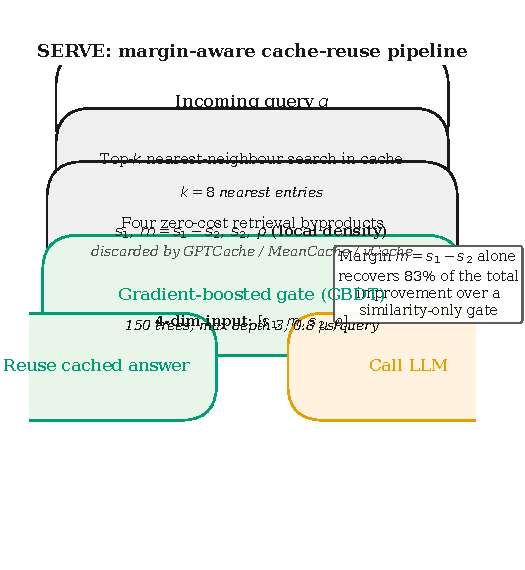
\includegraphics[width=\columnwidth]{figures/fig1_mechanism.pdf}
  \caption{SERVE intercepts a query, extracts similarity and margin from the cache, and feeds a 4-dimensional feature vector to a gradient-boosted gate that decides whether to reuse the cached answer or call the LLM.}
  \label{fig:fig1_mechanism}
\end{figure}

Query recurrence governs how much headroom the gate can exploit. Partitioning the test set by the fraction $r$ of queries that have a genuine duplicate anywhere in the cache reveals a monotonic pattern: SERVE's relative hit-rate gain over the fixed threshold at $\beta \le 1\%$ rises from +21.3\% at $r = 0.2$ (hit-rate $0.0233 \to 0.0283$), through +44.3\% at $r = 0.5$ ($0.0520 \to 0.0750$) and +69.9\% at $r = 0.7$ ($0.0654 \to 0.1110$), to +81.0\% at $r = 0.9$ ($0.0789 \to 0.1428$).
% E6
A denser pool of genuine duplicates, while producing better top-1 matches, also generates more near-duplicate collisions where both the first and second matches are highly similar yet semantically distinct. These collisions sit precisely in the low-margin region where $s_1$ alone is least informative, and where the gate's access to the margin dimension pays off most.

\begin{figure}[!t]
\centering
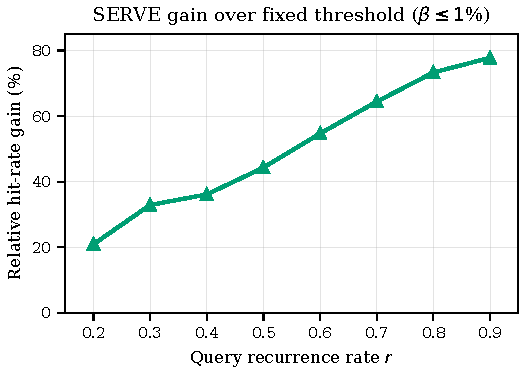
\includegraphics[width=\columnwidth]{figures/fig3_recurrence.pdf}
\caption{SERVE's absolute hit-rate advantage over the fixed threshold at $\beta \le 1\%$ grows monotonically as query recurrence rises, confirming that the gain concentrates where repeat traffic is heaviest.}
\label{fig:fig3_recurrence}
\end{figure}

The decision boundary learned by the gate explains the mechanism. Figure~\ref{fig:fig6_decision_boundary} visualizes the gate's behavior in the $(s_1, m)$ plane at $\beta \le 1\%$. The fixed threshold makes a vertical cut on $s_1$ alone. SERVE replaces that with a tilted effective boundary: it declines low-margin queries whose $s_1$ sits above the fixed cutoff and instead accepts high-margin queries whose $s_1$ falls below it. The pattern is geometric rather than heuristic. Queries the gate adds carry a substantially higher rate of correct serves than those it drops. The gate trades away marginal-similarity, low-confidence serves and buys back fewer, higher-confidence ones at the same budget.

\begin{figure}[!t]
\centering
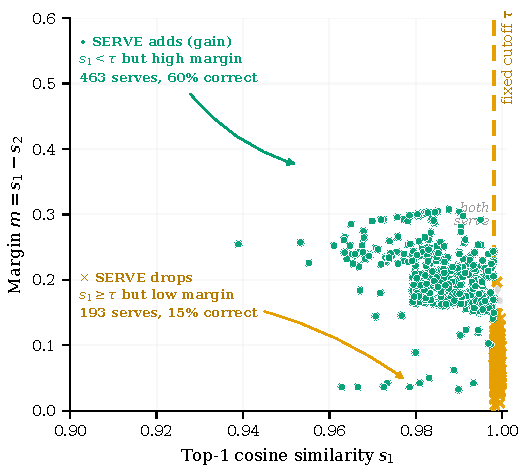
\includegraphics[width=\columnwidth]{figures/fig6_decision_boundary.pdf}
\caption{The learned decision boundary in the $s_1$-margin plane at $\beta \le 1\%$: SERVE accepts high-similarity, high-margin pairs and rejects low-margin ones that a similarity threshold would serve, trading quantity for quality at the same false-serve budget.}
\label{fig:fig6_decision_boundary}
\end{figure}

Feature ablation at $\beta \le 1\%$ measures what each dimension adds beyond raw similarity.
% E4
A gate using $s_1$ alone reaches a hit rate of $0.0292$.
% E4
Adding the margin lifts it to $0.0363$, a +24.4\% gain that recovers 83\% of the full four-feature improvement over similarity-only ($0.0378$).
% E4
The runner-up similarity $s_2$ adds +2.9\% (to $0.0374$), and local density $\rho$ contributes +1.1\% (to $0.0378$).
% E4
Removing the margin collapses the gate to near similarity-only performance because it encodes the ambiguity that scalar $s_1$ cannot resolve.

The margin advantage is not an artifact of encoder quality. On PAWS, an independently constructed adversarial paraphrase benchmark, the fixed similarity rule inverts below chance while SERVE, trained identically and with no sign knowledge, maintains a high AUC (Fig.~\ref{fig:fig5_paws}). The margin remains the dominant feature in the PAWS ablation as well. When the embedding model is upgraded from MiniLM (384d) to mpnet (768d), SERVE retains a comparable relative gain (Fig.~\ref{fig:fig2_embedding_quality}). A stronger encoder lifts both methods and leaves the edge essentially intact. The ambiguity that the margin measures reflects the query population's decision boundary, not encoder noise.

\begin{figure}[!t]
\centering
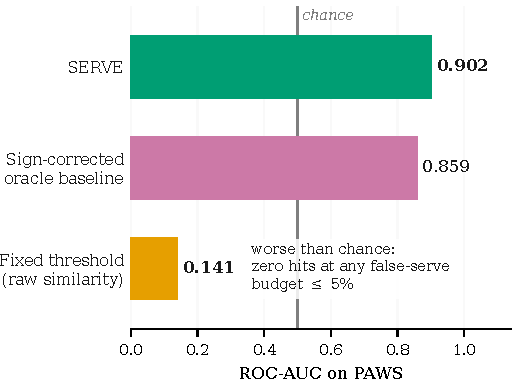
\includegraphics[width=\columnwidth]{figures/fig5_paws.pdf}
\caption{On the PAWS adversarial paraphrase benchmark, the fixed similarity rule inverts below chance while SERVE trained normally reaches high AUC, demonstrating robustness to embedding-space ambiguity that similarity alone cannot resolve.}
\label{fig:fig5_paws}
\end{figure}

\begin{figure}[!t]
\centering
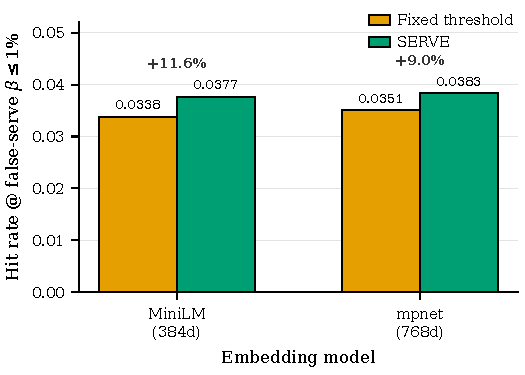
\includegraphics[width=\columnwidth]{figures/fig2_embedding_quality.pdf}
\caption{SERVE's relative gain over the fixed threshold persists when moving from MiniLM (384d) to the stronger mpnet (768d) encoder, confirming the margin signal is structural rather than an artifact of a weak embedding.}
\label{fig:fig2_embedding_quality}
\end{figure}

The trade-off frontier (Fig.~\ref{fig:fig2_frontier}, previous section) shows that SERVE's advantage concentrates at low false-serve budgets. At $\beta \le 5\%$, the gap narrows to near zero: when the operator tolerates one false serve in twenty, even a crude threshold serves nearly everything plausible and the gate has little discriminative headroom. The entire case for margin-aware gating rests on the strict-budget regime. The recurrence$\times$budget grid in Fig.~\ref{fig:fig4_best_regime_grid} characterizes precisely when the approach earns its keep: high recurrence and a strict false-serve budget compound, producing $2.6\text{--}3.15\times$ the served hits of the fixed threshold in the strictest cells tested. Figure~\ref{fig:fig4_grid} confirms the pattern across the full parameter space: gain rises along both axes independently and sharpens where they intersect. The regime where SERVE provides the largest benefit, tight reliability constraints combined with sustained repeat traffic, is the regime most plausibly associated with FAQ and customer-support caches.

\begin{figure}[!t]
\centering
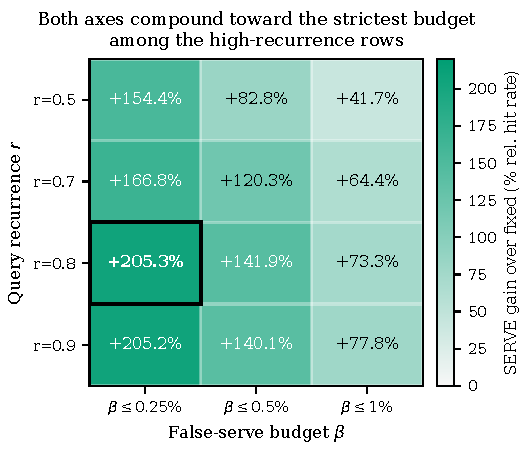
\includegraphics[width=\columnwidth]{figures/fig4_best_regime_grid.pdf}
\caption{The best regime grid maps SERVE's relative gain over the fixed threshold across query recurrence and false-serve budget: the advantage is largest under strict budgets with heavy repeat traffic, the conditions most characteristic of production caching.}
\label{fig:fig4_best_regime_grid}
\end{figure}

\begin{figure}[!t]
\centering
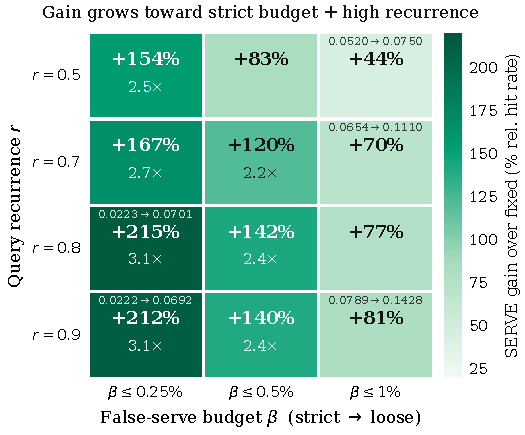
\includegraphics[width=\columnwidth]{figures/fig4_grid.pdf}
\caption{The full parameter grid confirms that SERVE's relative gain increases along both the recurrence and budget-strictness axes and compounds where they meet, with the highest-recurrence rows effectively tied at the strictest budget.}
\label{fig:fig4_grid}
\end{figure}

Two limitations bound the present study. All results come from two datasets (QQP, PAWS) and two embedding models (MiniLM, mpnet). Broader evaluation across additional domains (code search, multilingual, retrieval-augmented-generation corpora) and embedding families remains future work. The high-recurrence regime characterization is constructed by direct manipulation of $r$ in the test-query population rather than measured from production traffic. The gate is retrained per cache configuration rather than updated online as cache content drifts.

For deployment, the practical path is straightforward. The gate's four features are byproducts of the top-$k$ nearest-neighbor search the cache already performs. Training the gate once on a small, representative set of query pairs yields a model that runs in under a microsecond per query and requires no change to the cache backend or retrieval infrastructure. The operator selects a false-serve budget, trains the gate once, and earns improved hit rates at no additional retrieval cost, with the payoff concentrated in the regime where it matters most.